\subsection{Life in the Universe}
Life on earth started ~3.85 billion years ago shortly after a heavy bombardment as fossils and carbon dating imply. Fossiles tend to be found in sedimentary rock.

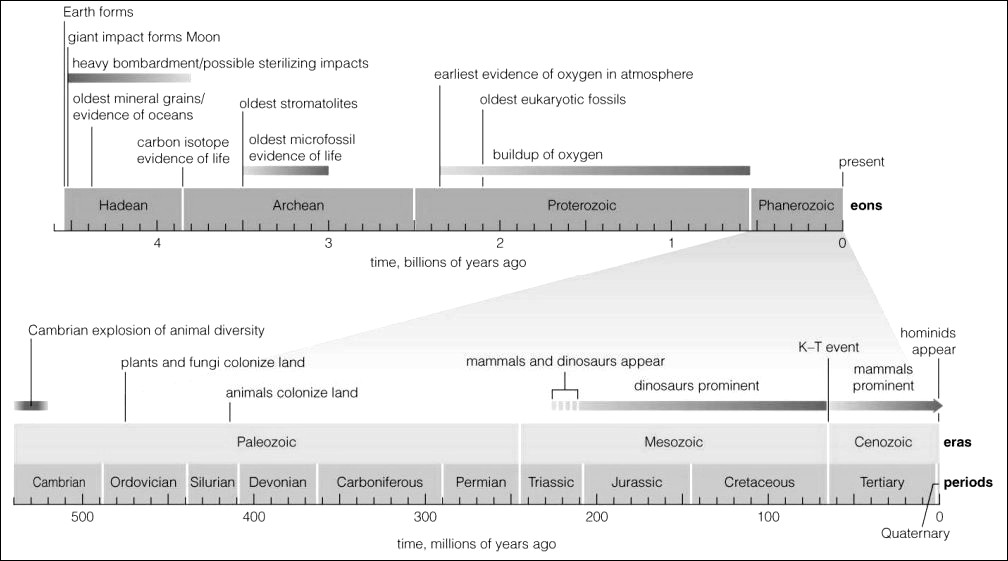
\includegraphics[angle=90,scale=0.7]{geologicalTimeline}

We all know that life came about through evolution. Genetics builds a tree of life through relationships that implies a common ancestor for all life probably similar to bacteria found deep in the ocean near volcanic vents. We still dont know how that common ancestor came to be. The Miller-Urey experiment (among others) shows that the building blocks of life can arise spontaneously under the conditions of early earth.

Chemicals to Life:
\begin{enumerate}
\item Naturally forming organic molecules are building blocks of life
\item Clay minerals catalyze production of RNA and membranes that form pre-cells
\item Molecular natrual selection favors efficient self-replicating RNA molecules
\item True living cells with RNA genome give rise to RNA world
\item DNA evolves from RNA and biological evolution continues
\end{enumerate}

One idea is that live could have come from another planet (Venus, Earth, and Mars exchanged tones of rock and some microbes can survive for years in space).

Brief History of life:
\begin{itemize}
\item 4.4 billion years - early oceans form
\item 3.5 billion years - cyanobacteria start releasing oxygen
\item 2.0 billion years - oxygen begins building up in atmosphere
\item 540–500 million years - Cambrian Explosion
\item 225–65 million years - dinosaurs and small mammals (dinosaurs ruled)
\item Few million years - earliest hominids
\end{itemize}

Oxygen didn't always exist so readily on earth. The evolution of \textbf{cyanobacteria} kicked it off by releasing oxygen to the atmosphere using photosynthesis.

(Bear)Necessity of Life:
\begin{itemize}
\item nutrient source
\item energy
\item liquid water
\end{itemize}

\subsubsection{Life on Other Planets}
Erosion lines on mars imply that it had liquid water in its distant past, there is still subsurface ice would could result in near surface water near its volcanoes. The Curiosity rover landed on mars to investigate the habitability of the planet.

Another potential is the moon \textbf{Europa} which we think has a layer of liquid water or warm convecting ice. Two other Jupiter moons, \textbf{Ganymede} and \textbf{Callisto} also show evidence of subsurface oceans. Very little energy reaches these moons, but life may be possible.

The moon \textbf{Titan} is much too cold for liquid water (there may be some deep under the surface) but it does have lakes of liquid methane.

\textbf{Encelandus} has ice foundations that suggest it may have a subsurface ocean.

\subsubsection{Life Outside our Solar System}
Habitable Solar System:
\begin{itemize}
\item old enough to allow time for evolution (no high mass stars, too young, 1\% of systems)
\item need to have stable orbits (might rule out multistar systems, 50\% of systems)
\item must have habitable zone (place where planets of the right size could have liquid water), larger stars have larger zones
\end{itemize}
There are billions of stars in the milky way alone that fulfill the above constraints.

It is very hard to spot a earth like planet due to their size and distance from their star (see previous section on finding extrasolar planets for a better explanation). We launched Kepler specifically to look at 100,000 stars for habitable planets and future inferometers may be precise enough to see earth-sized planets.

We can also use spectrometry to see the composition of planets to determine if they have the elements necessary for life.

\subsubsection{Earth-like Planets}
Some scientists argue that the proportions of heavy elements need to be just right for the formation of habitable planets. If so, then Earth-like planets are restricted to a galactic habitable zone.

Some scientists argue that the proportions of heavy elements need to be just right for the formation of habitable planets. If so, then Earth-like planets are restricted to a galactic habitable zone.

Some scientists argue that plate tectonics and/or a large moon are necessary to keep the climate of an Earth-like planet stable enough for life.

We dont know how important the above concerns are so its very hard to make a guess as to how common earth-like planets are and how many would be habitable.

\subsubsection{The Search for Extraterrestrial Intelligence}
The drake equation tries to calculate how many civilization we could communicate with exist
\begin{center}
    $N_{HP} \times f_{life} \times f_{civ} \times f_{now}$
\end{center}
$N_{HP}$ = total number of habitable planets in galaxy = probably billions\\
$f_{life}$ = fraction of habitable planets with life = hard to say (near 0 or 1)\\
$f_{civ}$ = fraction of life-bearing planets with civilization at some time = took 4 billion years on earth \\
$f_{now}$ = fraction of civilizations around now = depends on if civilizations survive long-term

Humans are not very exceptional (not too far from a line of best fit) in our brain mass to body mass ratio.

SETI is designed to look for deliberate signals from extraterrestrial civilizations and even to send some messages of our own.

\subsubsection{Interstellar Travel and Communications}
Current spacecrafts travel at one ten thousandth of the speed of light which means it would take a ridiculous amount of time to get to the nearest stars. We sent a message out with Voyager in hopes of reaching one someday.

Problems with space travel:
\begin{itemize}
\item Far more efficient engines are needed.
\item Energy requirements are enormous.
\item Ordinary interstellar particles become like cosmic rays.
\item Social complications of time dilation.
\end{itemize}

\textbf{Fermi's paradox} suggests that civilizations should be very common in our galaxy so why haven't we found any.

Explanations:
\begin{itemize}
\item  life/civilization is much rarer than we might have guessed
\item Civilizations are common, but interstellar travel is not
\begin{itemize}
\item interstellar travel is more difficult than we think.
\item the desire to explore is rare.
\item civilizations destroy themselves before achieving interstellar travel.
\end{itemize}
\item we just haven't met them yet
\end{itemize}
